\documentclass[tikz,border=6pt]{standalone}
% Shared visual language for the book's standalone vector figures.
% Keep this file compatible with the TeX Live version used by LyX.
\usepackage{amsmath,amssymb}
\usepackage{array,booktabs}
\usepackage{pgfplots}
\usepackage{pgfplotstable}
\usetikzlibrary{arrows.meta,calc,positioning}
\pgfplotsset{compat=1.17}

\definecolor{BookBlue}{HTML}{0072B2}
\definecolor{BookOrange}{HTML}{D55E00}
\definecolor{BookGreen}{HTML}{009E73}
\definecolor{BookGray}{HTML}{666666}
\definecolor{BookLightGray}{HTML}{D9D9D9}

\pgfplotsset{
  book axis/.style={
    axis line style={black!75,line width=0.55pt},
    tick style={black!75,line width=0.45pt},
    tick label style={font=\small},
    label style={font=\small},
    legend style={
      font=\small,
      draw=none,
      fill=none,
      cells={anchor=west},
    },
    grid style={BookLightGray,line width=0.35pt},
    major grid style={BookLightGray,line width=0.35pt},
  },
}

\begin{document}
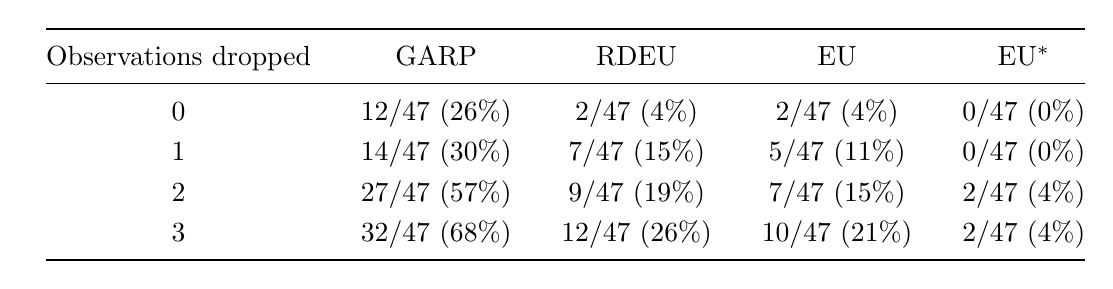
\begin{tikzpicture}
  \node[inner sep=0pt] {
    \renewcommand{\arraystretch}{1.22}
    \setlength{\tabcolsep}{9pt}
    \begin{tabular}{@{}ccccc@{}}
      \toprule
      Observations dropped & GARP & RDEU & EU & EU$^{*}$ \\
      \midrule
      0 & 12/47 (26\%) & 2/47 (4\%)  & 2/47 (4\%)  & 0/47 (0\%) \\
      1 & 14/47 (30\%) & 7/47 (15\%) & 5/47 (11\%) & 0/47 (0\%) \\
      2 & 27/47 (57\%) & 9/47 (19\%) & 7/47 (15\%) & 2/47 (4\%) \\
      3 & 32/47 (68\%) & 12/47 (26\%)& 10/47 (21\%)& 2/47 (4\%) \\
      \bottomrule
    \end{tabular}
  };
\end{tikzpicture}
\end{document}
